\documentclass[11pt,a4paper]{article}
\usepackage[margin=1in]{geometry}
\usepackage{amsmath,booktabs,graphicx,hyperref}
\title{Full manuscripts and shared theory: a first Topic E audit}
\author{Human Compression project}
\date{11 October 2026}
\begin{document}
\maketitle
\section{What is compared}
The intake is Leemans and Schulte's \emph{Groups of type $L_2(q)$ acting on
polytopes} (L083) and \emph{Polytopes with groups of type $\mathrm{PGL}_2(q)$}
(L079). Their declared main results classify the regular polytopes of rank
at least four with these groups. Our replacement is the complete common
theory $U_E$ and its two complete applications $A_1,A_2$, together with the
required program for the ten universal presentations.

The exact source PDFs and all earlier proof admissions are bound in the
accompanying JSON records. The L083 contract includes the rank restriction,
the unique marked 11-cell and 57-cell, the universal table and their stated
geometry. L079's Theorem 10 gives the unique marked 4-simplex. Its
seventeen-case semilinear census and subsequent conjecture are ancillary
to that expressly stated main theorem and are not recovered here.
Other background and chiral discussions are likewise outside the
contracts. Their text is nevertheless counted in the full-source lengths.
This comparison concerns recovery of the main results, not every assertion.

\section{Lengths and complete acquisition cost}
The primary ruler is the number of NFC-normalized, non-whitespace
characters extracted by pypdf 6.13.0. We include every source page,
including titles, introductions, ancillary material and references,
removing only explicitly identified repeated page furniture. All of
$U_E,A_1,A_2$ is charged, without removing the shared theory from the
total. The program is counted through its complete rendered appendix,
in the same units.

\begin{center}
\begin{tabular}{lr}
\toprule Document or artifact & Characters\\\midrule
Full source L083 & 20,885\\
Full source L079 & 20,908\\
Complete common theory $U_E$ & 18,264\\
Application $A_1$ & 8,213\\
Application $A_2$ & 5,737\\
Required shared program & 4,754\\\bottomrule
\end{tabular}
\end{center}
Thus the full-manuscript written comparison is
\[
 \frac{20\,885+20\,908}{18\,264+8\,213+5\,737}
 =\frac{41\,793}{32\,214}=1.297355\ldots.
\]
Charging our required program gives the known-cost comparison
\[
 \frac{41\,793}{32\,214+4\,754}
 =\frac{41\,793}{36\,968}=1.130518\ldots.
\]
The historical program cost is unknown, so the latter is not an exact
all-artifact ratio. Classical external inputs remain explicitly retained;
no unconditional library cost or minimum proof length is measured.
Conditional on acquiring the complete common theory and shared program,
the local factors are $20\,885/8\,213=2.5429\ldots$ and
$20\,908/5\,737=3.6444\ldots$.

\section{Sensitivity and the cumulative comparison}
The older factor $0.835226\ldots$ used selected principal-proof passages
as the source numerator: $26\,906/32\,214$. It answers a narrower question
and remains visible. In particular, the present full-manuscript saving
does not establish that our proofs are shorter than those selected source
proofs. Across all five fixed text metrics and both NFC and NFKC
normalizations, the full-manuscript written factors range from
$1.297$ to $1.552$; the corresponding comparisons including our required
program range from $1.131$ to $1.403$. These are extraction sensitivities,
not confidence intervals.

The source PDFs contain 14 and 9 pages; our papers contain 7, 3 and 2
pages, plus a three-page program appendix. Different typography makes
page counts supplementary observations rather than the primary ruler.
All six PDFs have been checked for nonprinting control characters,
replacement characters and private-use characters in their extracted text.

\begin{center}
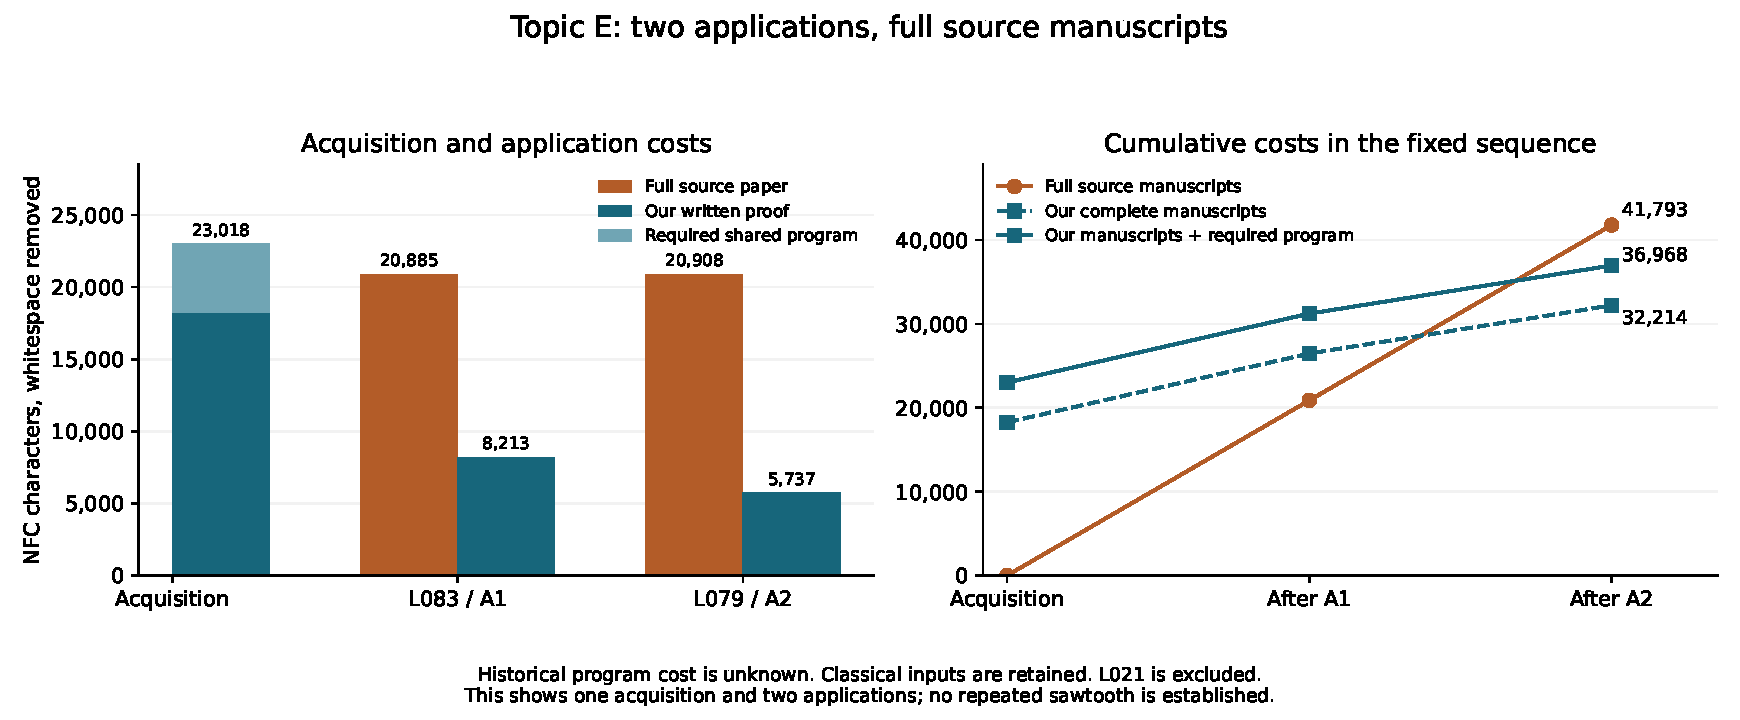
\includegraphics[width=\textwidth]{costs.pdf}
\end{center}
The full acquisition is $18\,264+4\,754=23\,018$. After the two applications,
our cumulative known costs are $31\,231$ and $36\,968$, compared with
source lengths $20\,885$ and $41\,793$. The second application repays
the measured acquisition under this full-manuscript comparison. There
is one acquisition and two applications; a repeated sawtooth pattern
has not been established.

\section{Audit scope and remaining work}
The author measurement and two independent recounts agree. Root's
recount recognizes each page header or footer directly, without using
the author's extraction spans. All ten metric coordinates and all six
document text hashes agree; the complete required GAP program occurs
in the charged appendix. Source PDFs and extracted primary texts are
not redistributed. The protocol, code, measurements and reviews are
published alongside this note.

This audit retains the previously reviewed mathematical contracts. It
does not add source recoveries or open-question answers. The later L021
application is excluded: its complete costs and enlarged dependency
graphs still require review. The existing theorem graphs identify uses
of results, but a complete partition into individually weighted theorem
units remains unfinished. The next measurement must include that
application's new group-theoretic interface and required computation,
as well as all retained proof dependencies.
\end{document}
